
%%%%%%%%%%%%%%%%%%%%%%%%%%%%%%%%%%%%%%%%%%%%%%%%%%%%%%%%%%%
\section{experiment}\label{sec:expResults}
%%%%%%%%%%%%%%%%%%%%%%%%%%%%%%%%%%%%%%%%%%%%%%%%%%%%%%%%%%%

\begin{figure*}[!htb]
\centering
\renewcommand{\figwid}{0.38\columnwidth}
{
\begin{overpic}[width =\figwid]{twoR1.pdf}%\put(12,70){$t$  = 0 s}
\end{overpic}
\begin{overpic}[width =\figwid]{twoR2.pdf}\put(12,70){$t$  = 60 s}
\end{overpic}
\begin{overpic}[width =\figwid]{twoR3.pdf}\put(12,70){$t$  = 150 s}
\end{overpic}
\begin{overpic}[width =\figwid]{twoR4.pdf}\put(12,70){$t$  = 160 s}
\end{overpic}
\begin{overpic}[width =\figwid]{twoR5.pdf}\put(12,70){$t$  = 210 s}
\end{overpic}}
%\vspace{-3em}
\caption{\label{fig:storyReal}Position control of two kilobots (Alg. \ref{alg:XControl}) steered to corresponding colored circle. Boundary walls have nearly infinite friction, so the green robot is stopped by the wall from $t = 60$s until the commanded input is directed away form the wall at $t=150$s, while the pink robot in free-space is unhindered.}
\end{figure*}


%\subsection{Hardware System}


Our experiments are on centimeter-scale hardware systems called \emph{kilobots}.  These allows us to emulate a variety of dynamics, while enabling a high degree of control over robot function, the environment, and data collection. The kilobot, from \citet{Rubenstein2012,rubenstein2014programmable} is a low-cost robot designed for testing collective algorithms with large numbers of robots. It is available as an open source platform or commercially from~\citet{K-Team2015}.  Each robot is approximately 3 cm in diameter, 3 cm tall, and uses two vibration motors to move on a flat surface at speeds up to 1 cm/s.  Each robot has one ambient light sensor that is used to implement \emph{phototaxis},  moving towards a light source. 
In these experiments as shown in Fig.~\ref{fig:setup}, we used $n$=100 kilobots, a 1 m$\times$1 m whiteboard as the workspace, four 30W and four 50W LED floodlights arranged 1.5 m above the plane of the table at the $\{N,NE,E,SE,S,SW,W,NW\}$ vertices of a 6 m square centered on the workspace. The lights were controlled using an Arduino Uno board connected to an 8-relay shield.  Above  the table, an overhead machine vision system tracks the position of the swarm.


\begin{figure}
\begin{center}
	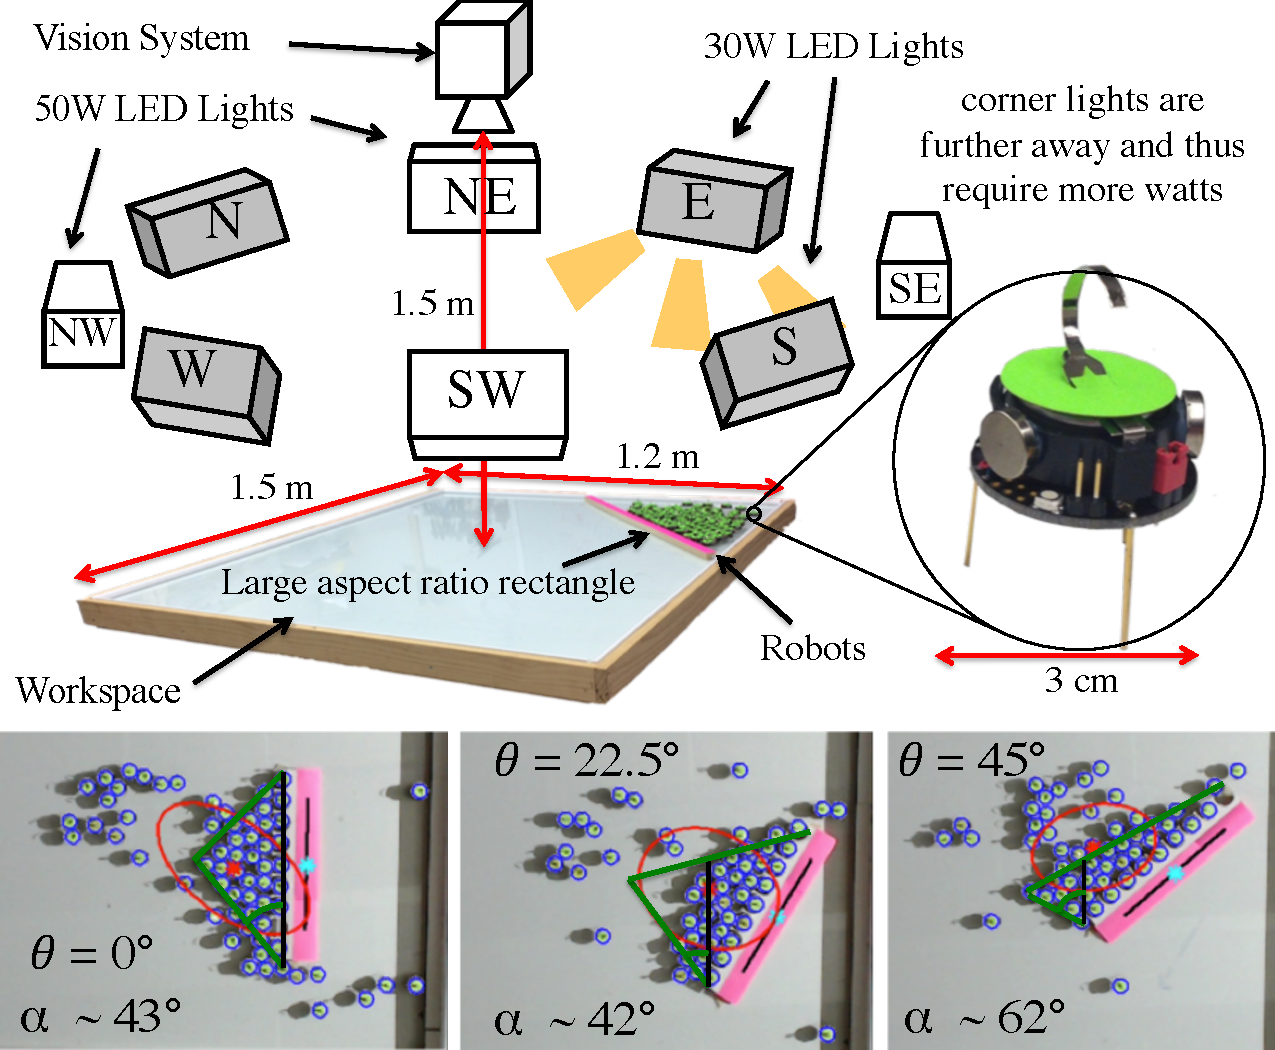
\includegraphics[width=.9\columnwidth]{SetUp.pdf}
\end{center}
\vspace{-1em}
\caption{\label{fig:setup}
Hardware platform:  table with 1$\times$1 m workspace, surrounded by eight remotely triggered LED floodlights, with an overhead machine vision system.
}
\vspace{-1em}
\end{figure}
\subsection{Hardware Experiment: Position Control of Two Robots}
The walls of the hardware platform have almost infinite friction, due to a laser-cut, zigzag border and the three-legged design of the kilobots. When a kilobot is steered into the zigzag border, they pin themselves to the wall unless the global input directs them away from the wall.  This wall friction is sufficient to enable independent control of two kilobots, as shown in Fig.~\ref{fig:storyReal}.

\subsection{Hardware Experiment: Position Control of n Robots}


\subsection{Hardware Experiment: Control of Covariance}
To demonstrate covariance control $n$=100 robots were placed on the workspace and manually steered with lights, using friction with the boundary walls to vary the covariance from  -4000 to 4000 cm$^2$.  The resulting covariance is plotted in Fig.~\ref{fig:covExperiment}, along with snapshots of the swarm.




\begin{figure}
\begin{center}
	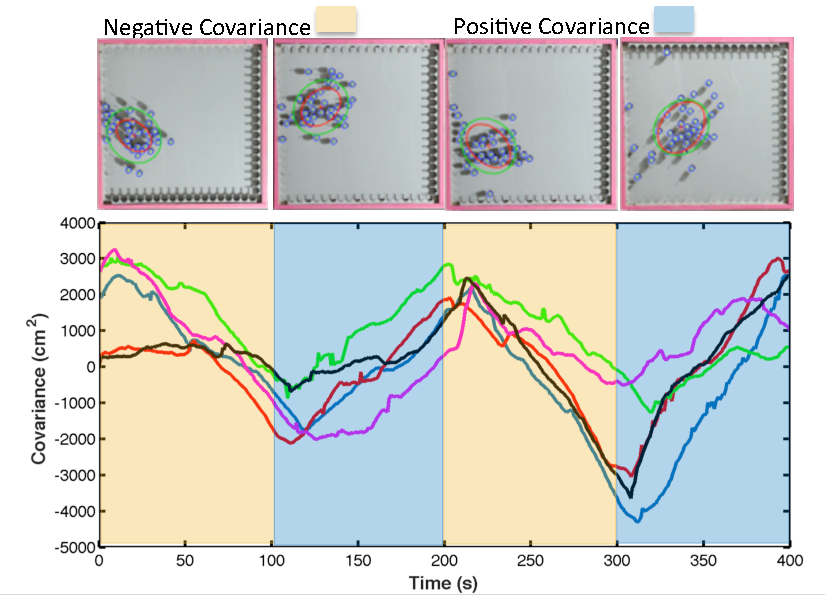
\includegraphics[width=\columnwidth]{newExperiment.pdf}
\end{center}
\vspace{-1em}
\caption{\label{fig:covExperiment}
Hardware demonstration steering 100 kilobot robots to desired covariance. The goal covariance is negative in first 100 seconds and is positive in the second 100 seconds. The actual covariance is shown in different trials. Frames above the plot show output from machine vision system and an overlaid covariance ellipse.
\vspace{-1em}
}
\end{figure}

